%%第二章,预备知识
\chapter{预备知识}
\label{chap:predefine}
序列比对领域常用的比对方法是对短读序列或者参考序列建立索引,除了前文所提到的通常的基于散列表的索引方法之外,最常使用的就
是压缩索引算法。压缩索引一方面能对数据规模进行压缩,减少算法实现时对内存空间的需求;另一方面也起到索引的作用,加快对模式的
搜索。如前文所述,DNA数据经过处理后可以当作一个文本序列,而序列比对问题可以抽象为一个模式查找问题,因此,序列比对使用的索
引方法本质上是文本索引算法。本章将介绍文本索引算法的一些概念,同时在第二部分对DNA数据格式处理做一些简述。

\section{压缩索引}
文本索引的目的是加快模式查询的速度。模式查询问题可以表述为:给定一个长为$m$的输入模式,找出$P$在长为$n$的文本$T$中的出现位置。
在模式查询领域,KMP提出了第一个时间复杂度为$O(m+n)$的线性查询算法,空间需求只有$O(1)$,这是非索引方法所能达到的最优结果。之
后为提高查询速度所涉及的搜索算法都是基于索引的方法。当前最优影响力的索引是倒排索引,但倒排索引是一种词索引,文本$T$必须
是结构化的,可以分为词,以便构建单词集。而如DNA等数据,是没有明显的单词集的,其所查询的模式也可能出现在文本$T$的任何一个
位置,即模式串$P$可以是$T$的任意子串。而后缀数组和后缀树以及类似trie树或者自动机都可用于DNA这样的无结构文本的模式查询,这
种索引称为全文本索引(full text index)。

后缀数组和后缀树由于其所需存储空间过大,在实践应用中存在诸多限制,而压缩索引的出现就是针对全文本索引空间复杂度过高的一个解决
方案。最有名的两个全文本压缩索引就是压缩后缀数组和FM索引。这两个索引的优势还体现在其自索引性质上,即建立索引后,无需再保存
原文本$T$,CSA或者FM本身即隐含了文本$T$,这进一步使得索引的规模降到了文本的0阶经验熵。另一个问题是构建CSA或者FM时,都需要
$O(n\log n)$位的辅助空间,这使得在构建较大规模的文本(如本文中使用的人类基因组)索引时,对计算机内存的需耗很大,在常规PC上
无法完成索引构建工作,对此,Hon,Sadakane和Sung提出了逐步构建CSA和FM,再归并的方法\cite{lam2002space}\cite{hon2003constructing},
使得构造空间降低到了$O(n\log |\Sigma|)$位。

以BWT为代表的自索引算法近年来在序列比对领域多有出现,例如前文中提到的Bowtie,BWA等。本文提出的序列比对算法则使用另一种自索引
算法:压缩后缀数组(CSA)\cite{grossi2005compressed}。同BWT相比,CSA的模式查询速度更快,应用于序列比对,相应的比对速
度也会更快,提高整个比对的效率。

CSA上的模式查询使用后向搜索算法(backward searching),Sadakane已经证明,在CSA上的后向搜索实践复杂度是$O(m)$,条件是字符集满足
$|\Sigma|=O(\text{poly} \log(n))$\cite{sadakane2002succinct}。本文提出的CSAA比对算法中,序列的查询也使用的是后向搜索算法。

\section{短读序列比对}

\subsection{DNA序列格式}

在DNA序列分析领域,DNA数据一般都来自国际知名的几大DNA数据库,如GenBanki,EMBL,DDBJ等。不同的测序方法,通常得到的序列数据也会
有一些差异。对此,为方便后续处理,生物信息学定义了一些通用的序列存储格式,如Fasta,Fastq等。通常Illumina测序数据都是Fastq格式,
所以本文中实现的软件CSAA也以Fastq作为标准输入格式。

Fastq格式是DNA序列格式中常见的一种,Fastq格式的序列一般都包含有四行,第一行由'@'开始,后面跟着序列的描述信息,这点跟Fasta格式
是一样的。第二行是序列的字符表示。第三行由'+'开始,后面也可以跟着序列的描述信息,和第一行信息相同,通常可以省略。第四行是第二行序列的质量评价
(quality values,是测序的质量评价),字符数跟第二行的序列是相等的。下面是Fastq格式序列的一个序列示例。

\begin{verbatim}
@HWUSI-EAS100R:6:73:941:1973#0/1
GATTTGGGGTTCAAAGCAGTATRRRGYKKKMSTCAAATAGTAAATCCATTTGTTCAACT
+HWUSI-EAS100R:6:73:941:1973#0/1
!''*((((***+))%%%++)(%%%%).1***-+*''))**55CCF>>>>>>CCCCCCC6
\end{verbatim}

Illumina测序仪是按照荧光信号来判断所测序的碱基是哪一种的,例如红黄蓝绿分别对应ATCG,但对每个结果都是有一定的误差的。最初sanger
中心用Phred quality score来衡量该read中每个碱基的质量,既$Q=-10\lg P$ ,其中$P$代表该碱基被测序错误的概率,如果该碱基测序
出错的概率为$0.001$,则$Q=30$,30+33=63,63对应的ASCii码为“?”,则在第四行中该碱基对应的质量分数代表值即为“?”。
一般地,碱基质量从0-40,既ASCii码为从 “!”(0+33)到“I”(40+33)。这上是sanger中心采用记录read测序质量的方法,Illumina
没有完全依照sanger中心的方法来定义测序质量,而是把$P$换成了$P/(1-P)$,其他完全按照sanger的定义来做。可以看出当测序质量
很高的情况下两种形式几乎没区别,但低质量的碱基则有区别了。

在Fastq格式中还可能出现其他一些核苷酸符号,具体含义如表\ref{tab:tabatcg}所述。

\begin{table}[htbp]
    \caption{Fastq格式支持的核苷酸符号}
    \label{tab:tabatcg}
    \centering
    \begin{tabular}{ll}
        \hline\\
        核苷酸代码&意义\\
        \hline\\
        A & Adenosine \\
        C & Cytosine \\
        G & Guanine \\
        T & Thymidine \\
        U & Uracil \\
        R & G A (puRine) \\
        Y & T C (pYrimidine) \\
        K & G T (Ketone) \\
        M & A C (aMino group) \\
        S & G C (Strong interaction)\\
        W & A T (Weak interaction) \\
        B & G T C (not A) (B comes after A)\\
        D & G A T (not C) (D comes after C) \\
        H & A C T (not G) (H comes after G) \\
        V & G C A (not T, not U) (V comes after U)\\
        N & A G C T (aNy)\\
        X & masked \\
        - & gap of indeterminate length
    \end{tabular}
\end{table}

DNA序列的标准保存格式是Fastq等格式,同样的,对序列比对的输出格式,也有一个约定的标准数据格式:SAM格式。SAM的全称是
sequence alignment/map format,一般是文本形式的,也可以存为二进制形式文件,即BAM格式。SAM由头文件和map结果组成,头
文件由一行行以“@”起始的注释构成。而map结果是类似下面的文本:

\begin{verbatim}
C12FP66670 0    chr1  12805 1 42M4I5M * 0 0 TTGGATGCCCCTC...
C12FP30032 272  chr1  13494 1 51M     * 0 0 ACTGCCTGGCGCT...
\end{verbatim}

SAM文件中每个read只占一行,被tab分成了很多列,一共有12列,分别记录了:read名称,SAM标记,chromosome名称,5′端起始
位置,MAPQ(mapping quality,描述比对的质量,数字越大,特异性越高),CIGAR字串(记录插入,删除,错配信息),mate名称(
记录mate pair信息),mate的位置,模板的长度,read序列,read质量,程序用标记。

本文中重点关注的是第三列,chrome名称,以及第四列,起始位置。通常作为参考序列的基因组是由多条染色体构成的,比对程序
需要得到read在哪一条染色体上,以及在改染色体上的位置,即5'端起始位置。

\subsection{单端测序和双端测序}
目前的测序方法中,如Solid,都有单端测序(Single-read)和双端测序(Paired end)之分。二者再测序方法上不同,得到的测序数据也有一些
差异。主要区别在于文库的建立上。

无论是单端测序还是双端测序,第一步都是对DNA分子进行切割,这是通过切割酶来实现的。切割后,大DNA分子被切割成长为300bp左右的短
序列(fragments)。测序第二步是增值,通过对这些短序列进行复制,增值,提高DNA分子数量。第三部是加入引物,开始测序。单端测序时
只在DNA短序列分子的一端加上引物,然后依次读取核苷酸,直到读完一个read。通常一个read长为80到1000bp,读取核苷酸时,因为越往后
读取错误率越高,所以一般read序列也是越往后,可靠性越低。双端测序时,会在DNA短序列两端都加上引物,然后分别读取核苷酸。所以,
双端测序得到的是一个DNA短序列分子的两个read,这两个read读取的是DNA链的两个不同的链,并且因为只读取两端的前100bp左右的核苷酸,
所以,这两个read序列并不一定重合,二者之间有一定的距离(distance),distance的长度为短序列(fragment)的长度减去两个短读序列的
长度之和。反映到在参考DNA序列上,distance为两个序列映射位置之差的绝对值。

\subsection{DNA序列的预处理}
DNA序列的输入格式是Fastq,需要首先对其做一些预处理工作,将序列数据转成结构化的文本数据,以便使用CSA建立索引和比对。预处理
包括两部分数据的处理。处理方法类似。

首先建立索引时需要把参考序列处理成一个单串,因为参考序列会有多条序列组成,需要把这多条序列连接成一条序列,然后再建立索引。
预处理参考序列时要保存序列的辅助信息,这需要一个辅助的数据结构来完成。此外因为比对时的输入短读序列也需要保存其辅助信息,
所以预处理reads时一样要把核心的碱基序列提取出来,并用辅助数据结构保存reads的辅助信息。

\subsection{短读比对的过程}
短读序列比对是通过在一个参考序列中搜索一个模式,使得该模式和给定的短读序列尽量相似的过程。在比对的过程中,如果参考序列和
短读序列的两个核苷酸相同,称为一个匹配(match),如果不相同称为一个错配(mismatch)。错配一般有替换(substitute),插入(insert),
删除(delete)三种,后两者本质上都是让一个核苷酸和一个空位相匹配,所以插入和删除统称为空位比对(gap alignment)。如图\ref{fig:mismatch}
中,两个DNA序列的一个比对,图中上部分是参考序列的一个片段,下半部分是一个短读。这个匹配中,可以看到有多个错配(图中蓝色标记),
两个替换失配:G替换为C和A替换为T;还有两个gap匹配,C匹配一个gap,gap匹配一个T。在短读比对中,插入操作定义为在短读上插入一个
gap,而删除操作则定义为在参考序列上插入一个gap,这和在短读上删除一个核苷酸是等价的。由于参考序列建立索引后直接在参考序列上插
入gap是难以直接实现的,所以参考序列上的gap插入可以用read上的删除替代。

\begin{figure}[htbp]
    \centering
    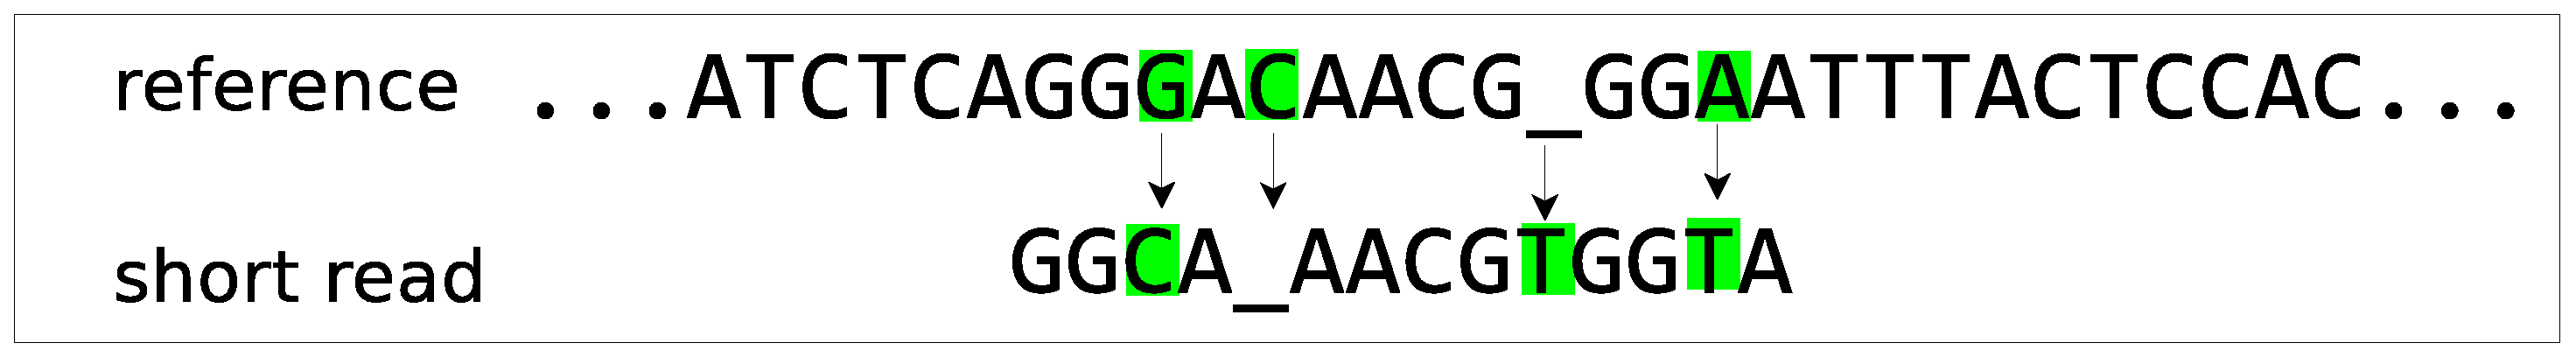
\includegraphics[width=0.9\textwidth]{mismatch.eps}
    \caption{短读比对示例} \label{fig:mismatch}
\end{figure}

\section{本章小结}
本章分为两个部分,对本文用到的一些先验知识做了一些简述。第一部分简述了索引,全文算引,自索引等概念,并对本文要用到的
索引算法:压缩后缀数组做了简介,描述了其特性,以及后向搜索。第二部分是对生物信息学领域序列
比对的一些基本概念的解释。包括DNA序列数据格式和单端测序,双端测序的概念。
